\documentclass{subfiles}

\begin{document}
\citet{cai2017mapping} demonstrates MAMMOTH-1 is in the density peak of BOSS1441 protocluster with overdensity $\rm \sigma=10.8 \pm 2.6$. \citet{arrigoni2018overdensity} finds the observed flux of BOSS1441 have good agreement with SED template of M82 which is a starburst galaxy. He estimates its far-infrared luminosity (rest-frame $\rm 8-1000\mu m$) $\rm L_{FIR}=3.2^{+7.4}_{-2.1} \times L_{\odot}$ which meets the criteria used to define ultra luminous infrared galaxy (ULIRG). Beside, the star-formation rate is also obtained by $\rm SFR=400 \ M_{\odot} \ yr^{-1}$. Based on the large SFR and the mass outflow rate $\rm \dot{M}_{out} \approx 500 \ M_{\odot} \ yr^{-1}$, we note that there should be a lot of gas injecting into the central AGN to supply the gas consumption. Furthermore, eight sources have been spectroscopically confirmed at $\rm z=2.32$ by our submillimeter observations \citep{qiongli2020} with our HST imaging even revealing three sources within $3\arcsec$. All of these evidences indicate that this is highly likely to be an violently interacting galaxy system.
	

We suggest that the physical picture of this area is like this: the three central sources are wildly interacting with each others. The middle source continues to accrete material from others to supply its SMBH growth, star formation and meanwhile producing strong outflow. Owing to the tidal effect between the three sources, a lot of material is pulled out from galaxies and densifies the gas environment which consequently lead to the quasar heavily obscured. This dense gas environment can also naturally explain why there is strong coupling between outflow and environment.
	\begin{figure*}
		\centering
		\subfloat{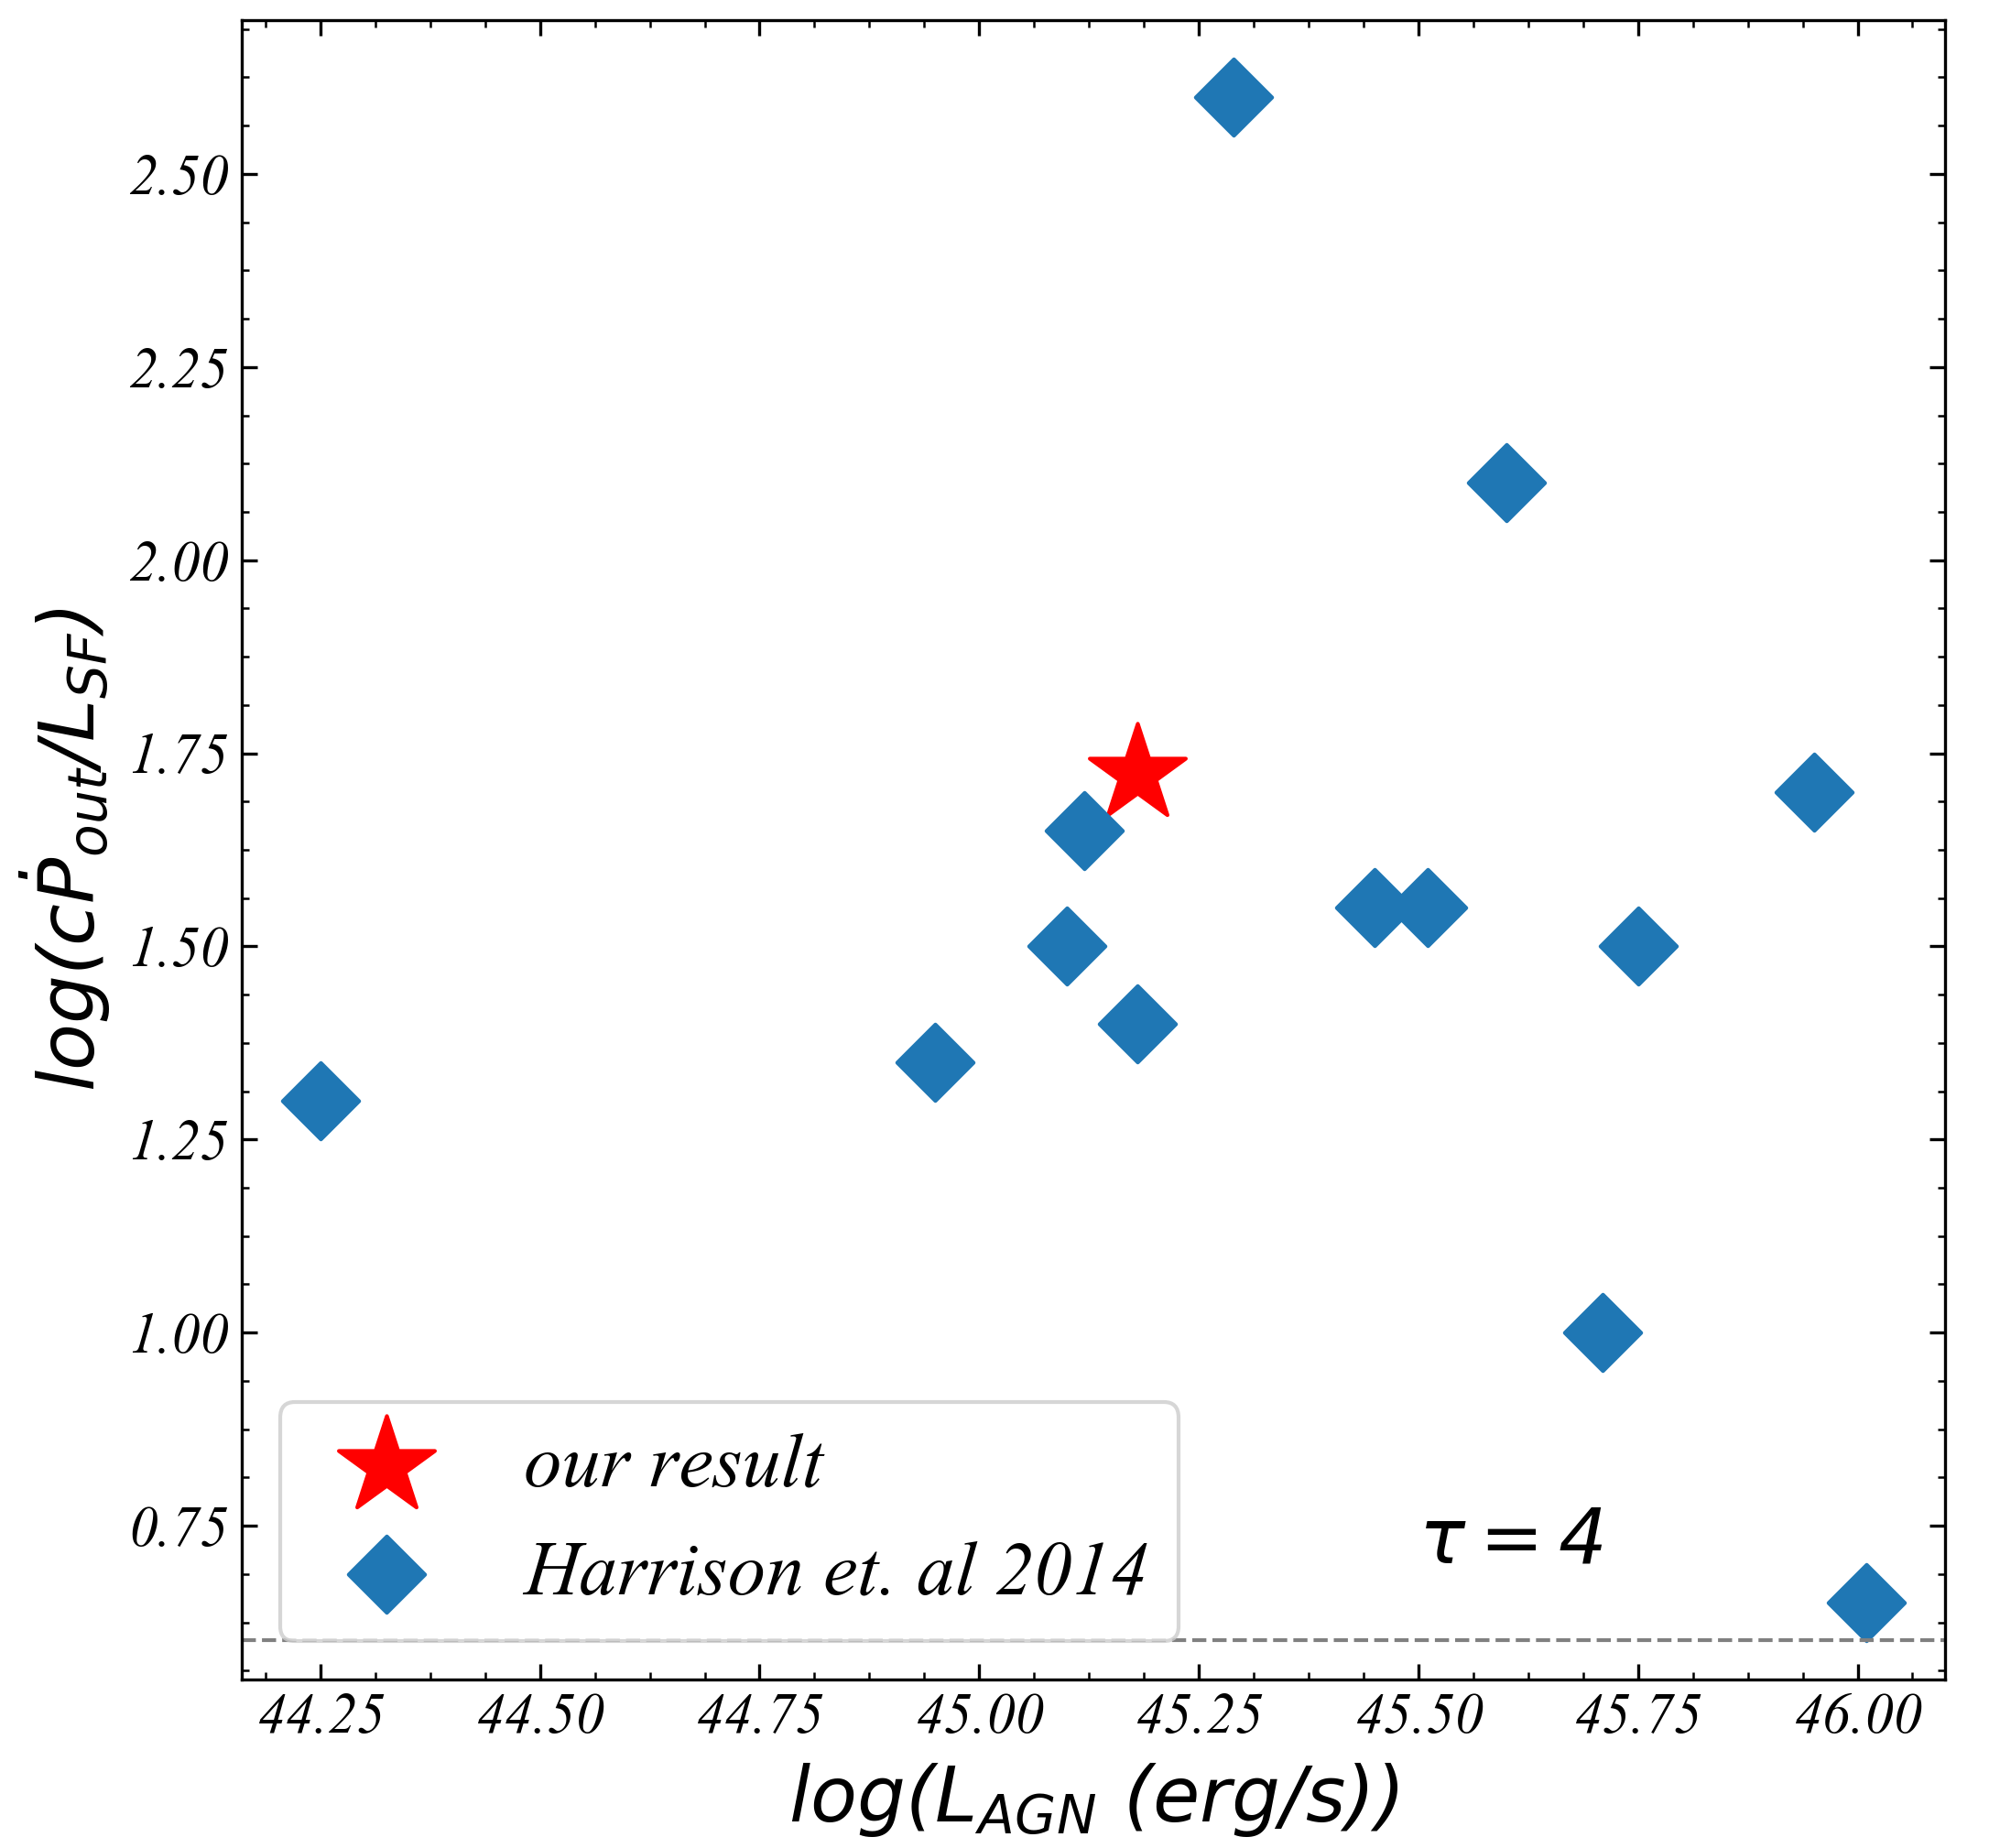
\includegraphics[width=0.5\textwidth]{figs/P_outSF_vs_L_AGN}}
		\subfloat{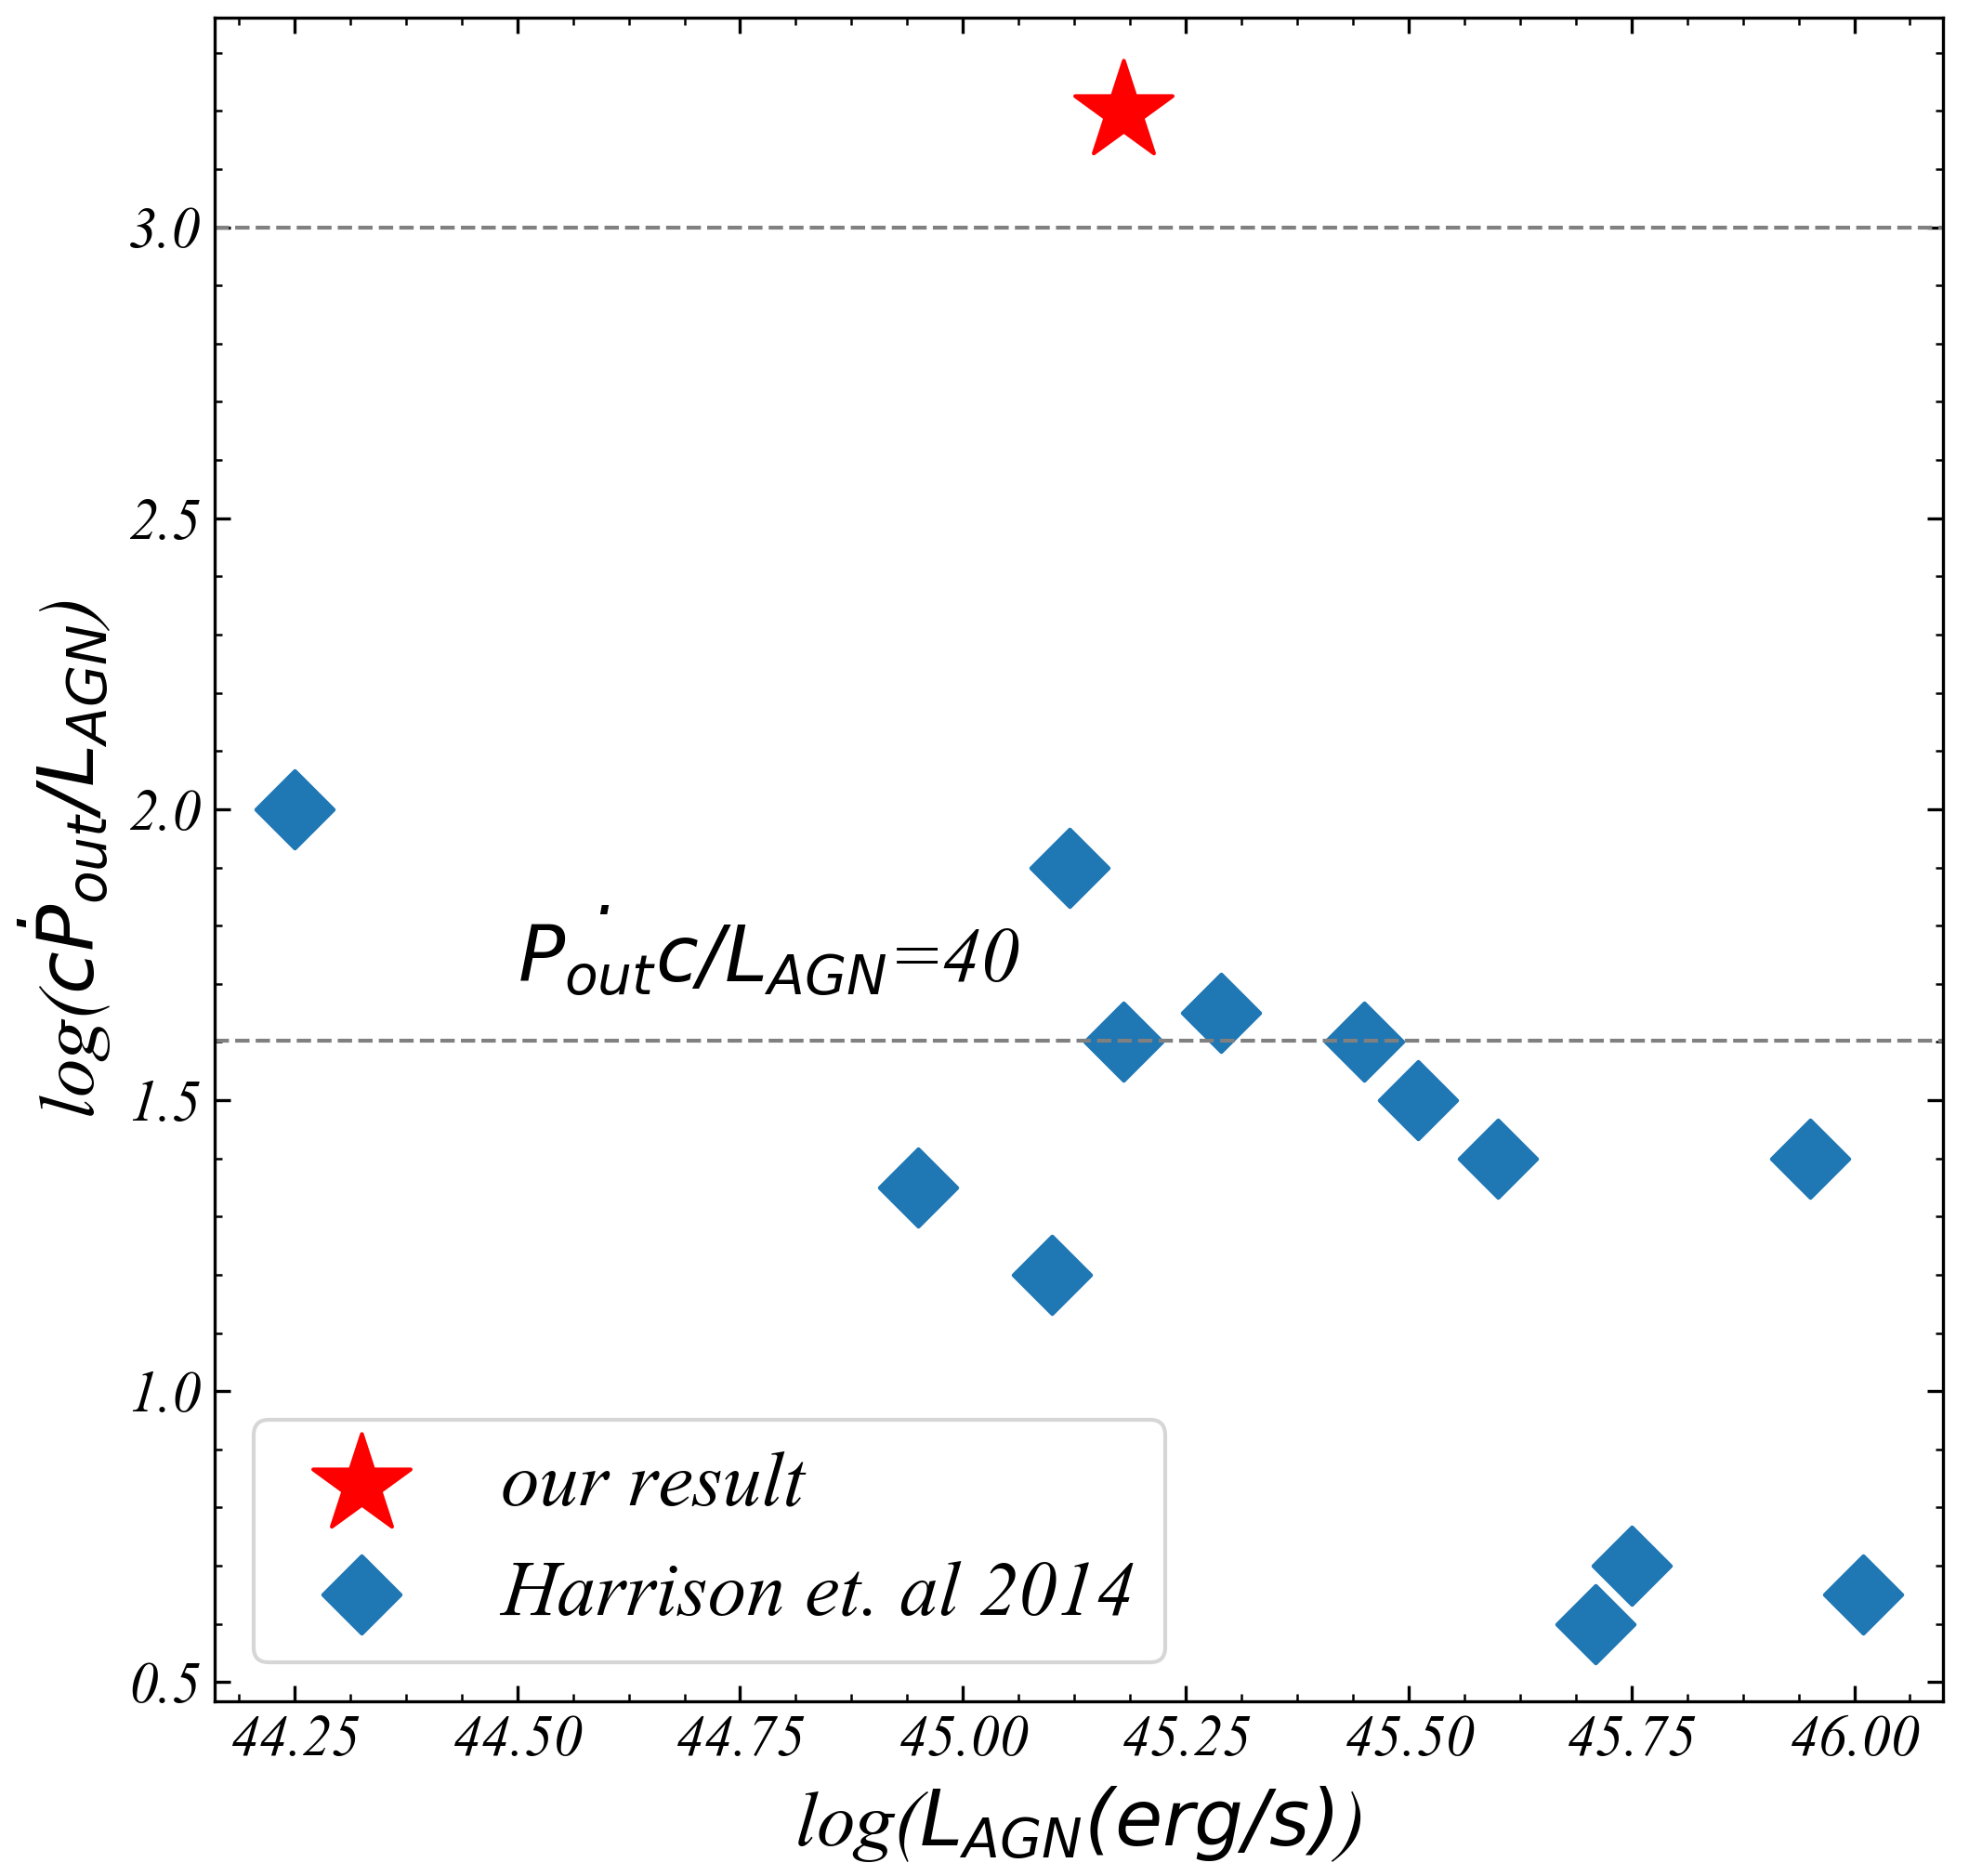
\includegraphics[width=0.5\textwidth]{figs/P_outAGN_vs_L_AGN}}
		\label{coupeffic}
		\caption{Left: momentum rates of the outflows($\dot{P_{out}}$ normalized to the star formation luminosity $L_{SF}/c$ versus AGN luminosity. The dashed lines represent the required optical depths if the outflows are driven by radiation pressure from star formation. Right: momentum rate of outflows normalized to AGN luminosity($L_{AGN}/c$) versus AGN luminosity. Based on our assumptions, the outflows are unlikely to be purely radiatively driven, the ratio is also to high for theoretical predictions of energy-driven outflows launched by AGN accretion-disc wind.}
	\end{figure*}
\end{document}